\documentclass[10pt]{article}
\usepackage[T1]{fontenc}

% Document Details
\newcommand{\CLASS}{AMATH 563}
\newcommand{\assigmentnum}{Sparse Regression}

\usepackage[margin = 1in, left=0.75in,right=0.75in]{geometry}
\usepackage{titling}
\setlength{\droptitle}{-6em}   % This is your set screw
\date{}
\renewcommand{\maketitle}{
	\clearpage
	\begingroup  
	\centering
	\LARGE \sffamily\textbf{\CLASS} \Large \assigmentnum\\[.8em]
	\large Tyler Chen\\[1em]
	\endgroup
	\thispagestyle{empty}
}
 % Title Styling


\usepackage{enumitem}

% Figures
\usepackage{subcaption}

% TikZ and Graphics
\usepackage{tikz, pgfplots}
\pgfplotsset{compat=1.12}
\usetikzlibrary{patterns,arrows}
\usepgfplotslibrary{fillbetween}

\usepackage{pdfpages}
\usepackage{adjustbox}

\usepackage{lscape}
\usepackage{titling}
\usepackage[]{hyperref}


% Header Styling
\usepackage{fancyhdr}
\pagestyle{fancy}
\lhead{\sffamily \CLASS}
\rhead{\sffamily Chen \textbf{\thepage}}
\cfoot{}

% Paragraph Styling
\setlength{\columnsep}{1cm}
\setlength{\parindent}{0pt}
\setlength{\parskip}{5pt}
\renewcommand{\baselinestretch}{1}

% TOC Styling
\usepackage{tocloft}
\iffalse
\renewcommand{\cftsecleader}{\cftdotfill{\cftdotsep}}

\renewcommand\cftchapafterpnum{\vskip6pt}
\renewcommand\cftsecafterpnum{\vskip10pt}
\renewcommand\cftsubsecafterpnum{\vskip6pt}

% Adjust sectional unit title fonts in ToC
\renewcommand{\cftchapfont}{\sffamily}
\renewcommand{\cftsecfont}{\bfseries\sffamily}
\renewcommand{\cftsecnumwidth}{2em}
\renewcommand{\cftsubsecfont}{\sffamily}
\renewcommand{\cfttoctitlefont}{\hfill\bfseries\sffamily\MakeUppercase}
\renewcommand{\cftaftertoctitle}{\hfill}

\renewcommand{\cftchappagefont}{\sffamily}
\renewcommand{\cftsecpagefont}{\bfseries\sffamily}
\renewcommand{\cftsubsecpagefont}{\sffamily}
\fi
 % General Styling
% Code Display Setup
\usepackage{listings,lstautogobble}
\usepackage{lipsum}
\usepackage{courier}
\usepackage{catchfilebetweentags}

\lstset{
	basicstyle=\small\ttfamily,
	breaklines=true, 
	frame = single,
	rangeprefix=,
	rangesuffix=,
	includerangemarker=false,
	autogobble = true
}


\usepackage{algorithmicx}
\usepackage{algpseudocode}

\newcommand{\To}{\textbf{to}~}
\newcommand{\DownTo}{\textbf{downto}~}
\renewcommand{\algorithmicdo}{\hspace{-.2em}\textbf{:}}
 % Code Display Setup
% AMS MATH Styling
\usepackage{amsmath, amssymb}
\newcommand{\qed}{\hfill\(\square\)}

%\newtheorem*{lemma}{Lemma} 
%\newtheorem*{theorem}{Theorem}
%\newtheorem*{definition}{Definition}
%\newtheorem*{prop}{Proposition}
%\renewenvironment{proof}{{\bfseries Proof.}}{}


% mathcal
\newcommand{\cA}{\ensuremath{\mathcal{A}}}
\newcommand{\cB}{\ensuremath{\mathcal{B}}}
\newcommand{\cC}{\ensuremath{\mathcal{C}}}
\newcommand{\cD}{\ensuremath{\mathcal{D}}}
\newcommand{\cE}{\ensuremath{\mathcal{E}}}
\newcommand{\cF}{\ensuremath{\mathcal{F}}}
\newcommand{\cG}{\ensuremath{\mathcal{G}}}
\newcommand{\cH}{\ensuremath{\mathcal{H}}}
\newcommand{\cI}{\ensuremath{\mathcal{I}}}
\newcommand{\cJ}{\ensuremath{\mathcal{J}}}
\newcommand{\cK}{\ensuremath{\mathcal{K}}}
\newcommand{\cL}{\ensuremath{\mathcal{L}}}
\newcommand{\cM}{\ensuremath{\mathcal{M}}}
\newcommand{\cN}{\ensuremath{\mathcal{N}}}
\newcommand{\cO}{\ensuremath{\mathcal{O}}}
\newcommand{\cP}{\ensuremath{\mathcal{P}}}
\newcommand{\cQ}{\ensuremath{\mathcal{Q}}}
\newcommand{\cR}{\ensuremath{\mathcal{R}}}
\newcommand{\cS}{\ensuremath{\mathcal{S}}}
\newcommand{\cT}{\ensuremath{\mathcal{T}}}
\newcommand{\cU}{\ensuremath{\mathcal{U}}}
\newcommand{\cV}{\ensuremath{\mathcal{V}}}
\newcommand{\cW}{\ensuremath{\mathcal{W}}}
\newcommand{\cX}{\ensuremath{\mathcal{X}}}
\newcommand{\cY}{\ensuremath{\mathcal{Y}}}
\newcommand{\cZ}{\ensuremath{\mathcal{Z}}}

% mathbb
\usepackage{bbm}
\newcommand{\bOne}{\ensuremath{\mathbbm{1}}}

\newcommand{\bA}{\ensuremath{\mathbb{A}}}
\newcommand{\bB}{\ensuremath{\mathbb{B}}}
\newcommand{\bC}{\ensuremath{\mathbb{C}}}
\newcommand{\bD}{\ensuremath{\mathbb{D}}}
\newcommand{\bE}{\ensuremath{\mathbb{E}}}
\newcommand{\bF}{\ensuremath{\mathbb{F}}}
\newcommand{\bG}{\ensuremath{\mathbb{G}}}
\newcommand{\bH}{\ensuremath{\mathbb{H}}}
\newcommand{\bI}{\ensuremath{\mathbb{I}}}
\newcommand{\bJ}{\ensuremath{\mathbb{J}}}
\newcommand{\bK}{\ensuremath{\mathbb{K}}}
\newcommand{\bL}{\ensuremath{\mathbb{L}}}
\newcommand{\bM}{\ensuremath{\mathbb{M}}}
\newcommand{\bN}{\ensuremath{\mathbb{N}}}
\newcommand{\bO}{\ensuremath{\mathbb{O}}}
\newcommand{\bP}{\ensuremath{\mathbb{P}}}
\newcommand{\bQ}{\ensuremath{\mathbb{Q}}}
\newcommand{\bR}{\ensuremath{\mathbb{R}}}
\newcommand{\bS}{\ensuremath{\mathbb{S}}}
\newcommand{\bT}{\ensuremath{\mathbb{T}}}
\newcommand{\bU}{\ensuremath{\mathbb{U}}}
\newcommand{\bV}{\ensuremath{\mathbb{V}}}
\newcommand{\bW}{\ensuremath{\mathbb{W}}}
\newcommand{\bX}{\ensuremath{\mathbb{X}}}
\newcommand{\bY}{\ensuremath{\mathbb{Y}}}
\newcommand{\bZ}{\ensuremath{\mathbb{Z}}}

% alternative mathbb
\newcommand{\NN}{\ensuremath{\mathbb{N}}}
\newcommand{\RR}{\ensuremath{\mathbb{R}}}
\newcommand{\CC}{\ensuremath{\mathbb{C}}}
\newcommand{\ZZ}{\ensuremath{\mathbb{Z}}}
\newcommand{\EE}{\ensuremath{\mathbb{E}}}
\newcommand{\PP}{\ensuremath{\mathbb{P}}}
\newcommand{\VV}{\ensuremath{\mathbb{V}}}
\newcommand{\cov}{\ensuremath{\text{Co}\VV}}
% Math Commands

\newcommand{\st}{~\big|~}
\newcommand{\stt}{\text{ st. }}
\newcommand{\ift}{\text{ if }}
\newcommand{\thent}{\text{ then }}
\newcommand{\owt}{\text{ otherwise }}

\newcommand{\norm}[1]{\left\lVert#1\right\rVert}
\newcommand{\snorm}[1]{\lVert#1\rVert}
\newcommand{\ip}[1]{\ensuremath{\left\langle #1 \right\rangle}}
\newcommand{\pp}[3][]{\frac{\partial^{#1}#2}{\partial #3^{#1}}}
\newcommand{\dd}[3][]{\frac{\d^{#1}#2}{\d #3^{#1}}}
\renewcommand{\d}{\ensuremath{\mathrm{d}}}

\newcommand{\indep}{\rotatebox[origin=c]{90}{$\models$}}




 % Math shortcuts

\usepackage{dblfloatfix}    % To enable figures at the bottom of page

% Problem
\newenvironment{problem}[1]{\vspace{2em}{\large\sffamily\textbf{#1}}\itshape\par}{}

\usepackage{nameref}
\newcommand{\vln}{\rotatebox{90}{--}}

\begin{document}

\twocolumn[{%
\begin{@twocolumnfalse}
\maketitle
\vspace{2em}
\begin{abstract}
We outline a sparse regression framework for finding a model given some data. This framework is implemented in Python and applied to two data sets. These examples demonstrate the difficulty of applying these methods to systems with limited data but yield results which encourage furture work.
%This report is bullshit, these methods are bullshit, my models are bullshit, nothing works, and nothing is grounded in any sort of understanding of what is going on.

\end{abstract}
\vspace{4em}
%\tableofcontents
%\vspace{3em}
\pagebreak\end{@twocolumnfalse}
}]

\section{Introduction and Overview}
The classic example of data science and data driven modeling is Johannes Keppler extracting the laws of planetary motion from data collected by Tycho Brahe. In the present we are able to gather and save a huge amount of data. As a result, techniques must be developed to extract useful information and models from this data. One such approach, explain in more detail in \cite{Brunton3932,lecture_notes}, is sparse regression. In this paper we outline the theoretical framework of sparse regression, implement such a framework in Python, and apply the framework to two data sets.

\section{Theoretical Background}

\subsection{Sparse Regression}
Suppose we have data \( d\in\RR^m \) for which we would like to find a model. Rather than picking a model ahead of time and ``imposing'' it on our data, we can construct a more general ``library'' of functions \( f_i \in \RR^{m} \), \( i=1,2 \cdots, n \) (each possibly depending on \( d \)) from which to pick our model used to represent \( d \). We take the model \( y \) to be a linear combination of of these functions with coefficients \( c\in\RR^{n} \).
In some sense, a model which depends on fewer terms is desirable, and we can attempt to find such a model by promoting sparsity in the coefficients of the linear combination of our library functions.

Written in matrix form,
\begin{align*}
    \left[\begin{array}{cccc}
     \vln & \vln & & \vln \\
    f_1 & f_2 & \cdots & f_n \\
    \vln & \vln & & \vln
    \end{array}\right]
    \left[\begin{array}{c}c_1 \\ \vdots \\ c_n\end{array}\right]
    \approx
    \left[\begin{array}{c}d_1 \\ \vdots \\ d_m \end{array}\right]
\end{align*}

In practice this will be an overdetermined system as we will have many samples in \( d \) but hope to find a ``simple'' model. The classic way to solve an overdetermined system is least squares regression. However, since least squares gives a relatively ``balanced'' weighting to all of the functions in the library, the coefficients chosen will almost certainty all be nonzero. As a result, we would like to find a method of solving the overdetermined system which will force some coefficients to be zero.

We can generalize the least squares problem as finding \( c\in\RR^n \) which, for a fixed \( A \) and \( d \), solves the minimization problem,
\begin{align}
    \min_{c\in\RR^n} g(A,d,c)
\end{align}

A common choice for \( g \) is,
 \begin{align}
    g(A,d,c) &= \dfrac{1}{2}\norm{d-Ac}_2^2 + \lambda \norm{c}_1 \label{lasso}
\end{align}
When \( \lambda = 0 \) this is the standard least squares fit. For \( \lambda > 0 \), extra weight is placed on the sparsity of the solution. This is commonly referred to as least absolute shrinkage and selection operator (lasso).

\subsection{KL Divergence, AIC, BIC}
Once we have constructed a model, \( y \), we would like to know how ``good'' of a model it is. We use three metrics, KL divergence, AIC, and BIC, to measure how accurate our models are. We pull much of our methodology in this section from Chapters 1 and 2 of \cite{Burnham}.%\textit{Model Selection and Multimodel Inference: A Practical Information-Theoretic Approach} \cite{Burnham}.

Given two (discrete) probability distributions \( P \) and \( Q \) we define the KL divergence,
\begin{align}
    \text{KL}(P,Q) = \sum_i P(i) \log \left( \dfrac{P(i)}{Q(i)} \right) \label{kl}
\end{align}

This is a measure of the information lost when \( Q \) is used to approximate \( P \).


We make the assumption that the residuals \( d_i - y_i \) are i.i.d. normal random variables with mean zero. Defining, \( \text{RSS} = \norm{d_i - y_i}_2^2 \) and variance of these residuals, \( \sigma^2 = \text{RSS} / n \), the maximum value of a model's log likelihood function is,
\begin{align}
    \ln\mL = -\dfrac{n}{2} \ln 2\pi - \dfrac{n}{2}\ln \sigma^2 - \dfrac{n}{2} \label{logl}
\end{align}

Denote the number of parameters in a model \( y \) with \( k \) and the number of data points with \( n \). We define the AIC and BIC scores,
\begin{align}
    \text{AIC}(d,y) &= 2k - 2\ln\mL \label{aic} \\
    \text{BIC}(d,y) &= k \ln n - 2\ln\mL \label{bic}
\end{align}

These scores penalize the use of more parameters and the use of more observations. This makes intuitive sense, since a simpler model which performs as ``well'' as a more complex one is desirable.

We make the note that what we take as our data depends on the analysis. For instance, even if we are given some data set, if we are doing sparse regression to find a model for the time derivative, we would use the time derivatives as the \( d_i \) described in (\ref{logl}).

This makes sense as even a perfect model with a slight error in the initial condition may vary wildly in position after some time, even if the derivatives (which is what were fit) are very accurate.

\subsection{Cross Validation}
In order to make sure our models represent the system we cross validate. Loosely speaking, this means we train a model on part of the data, and compare the prediction to some part of the data which was not used in training. This helps get a sense of how well the model will work on new data.

\subsection{Time Delay Embedding}
If we have a set of measurement for a system, one question is how many hidden variables the system contains.
Broadly, time delay embedding hopes to recover the system's dimensionality.

We provide a simple example as intuition for this approach.
Consider the system of \( n \) coupled linear first order ODEs,
\begin{align}
    x' = Ax, && x(0) = x_0 \tag{ode}
\end{align}

If we numerically solve the system using forward Euler, we will have a system of \( n \) coupled difference equations,
\begin{align*}
    x^{(i+1)} = x^{(i)} + \d t Ax^{(i)}, && x^{(0)} = x_0 \tag{diff}
\end{align*}

Let \( x_j^{(k)} \) denote the \( j \)-th component of the \( k \)-th iterate. Consider the matrix,
\begin{align*}
    H = \left[\begin{array}{llll}
      x_j^{(0)} & x_j^{(1)} & \cdots & x_j^{(n)} \\
      x_j^{(1)} & x_j^{(2)} & \cdots & x_j^{(n+1)} \\
      \vdots & \vdots & & \vdots \\
      x_j^{(k)} & x_j^{(1+k)} & \cdots & x_j^{(n+k)}
    \end{array}\right]
\end{align*}

If \( k>n \) then the \( n+1 \)-th row can be written as a linear combination of the previous rows. This means there will be \( n \) nonzero singular values in the singular value decomposition (SVD) of \( H \).

Since this only requires a single component of the solutions in time, we make the observation that the dimensionality of the system can be recovered from just the solution \( x_j^{(k)} \), \( k=1,2,\ldots \).

Obviously this is a very simple system. Such an approach can be applied to more complex systems with varying degrees of success. In practice we found that even using other solving methods such as Runge-Kutta 4,5 to discretized the original system gave a Hankel matrix which had no clear cutoff in singular values even when very small time steps were used. That said, since we do not solve for the data used in the Hankel matrix, perhaps this does not matter.

\begin{figure*}[!b]
\begin{subfigure}[t]{.3\textwidth}\centering
  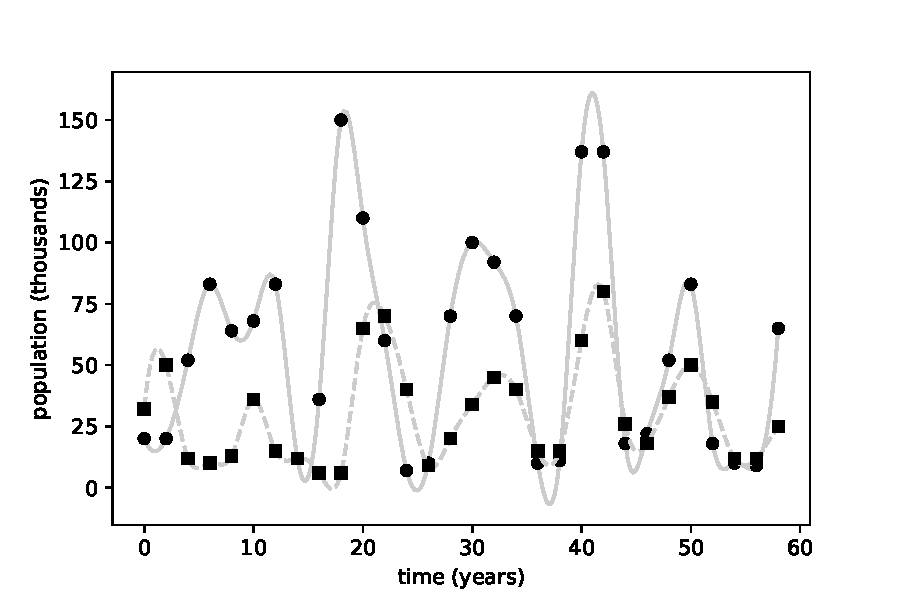
\includegraphics[width=\textwidth]{img/P/interp.pdf}
  \caption{circle: population (circle), lynx population (square), interpolated populations (grey)}
  \label{popvt}
\end{subfigure}\hfill
\begin{subfigure}[t]{.3\textwidth}\centering
  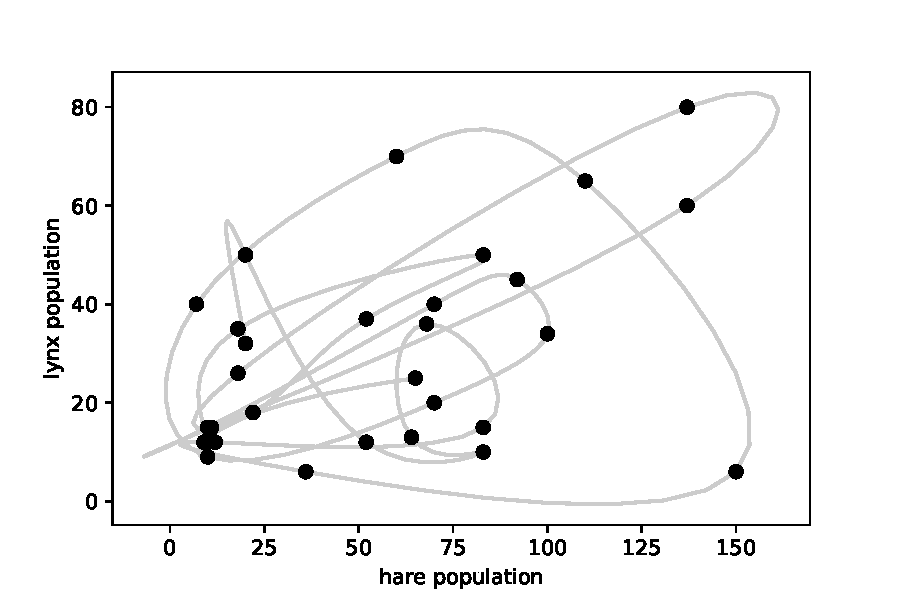
\includegraphics[width=\textwidth]{img/P/phase.pdf}
  \caption{phase diagram with interpolated populations (grey)}
  \label{popphase}
\end{subfigure}\hfill
\begin{subfigure}[t]{.3\textwidth}\centering
  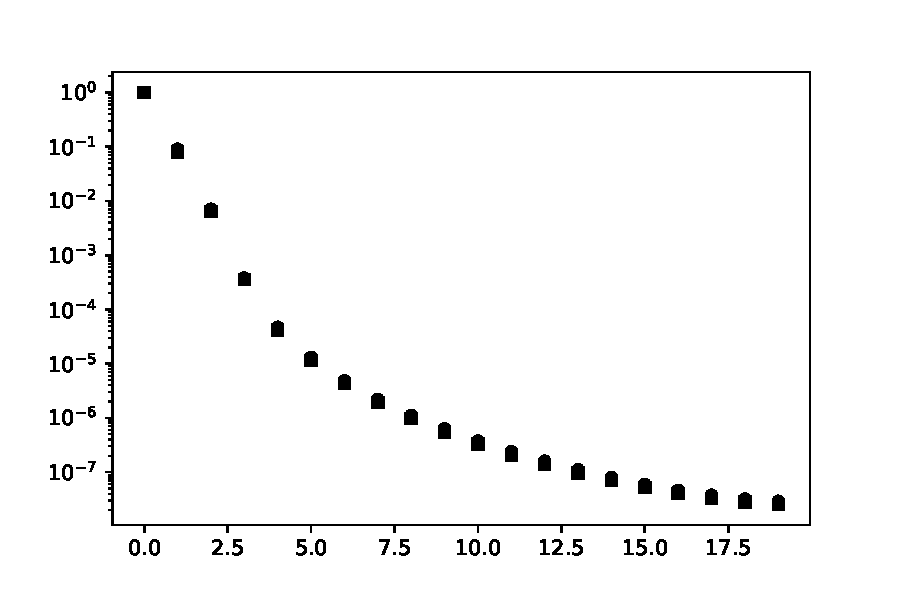
\includegraphics[width=\textwidth]{img/P/time_delay.pdf}
  \caption{singular values of time delay matrices (using data interpolated at 1451 points); hare (circle), lynx (square)}
  \label{hankel}
\end{subfigure}
\caption{}
\end{figure*}

\begin{figure*}[!t]\centering
\foreach \k in {100,200,500,211,222,511}{
\begin{subfigure}{.32\textwidth}
  \includegraphics[width=\textwidth]{img/P/\k.pdf}
  \caption{ {\tt m\k} }
\end{subfigure}
}
\caption{hare model (solid), lynx model (dashed)}
\label{models}
\end{figure*}


\section{Algorithm Implementation and Development}
The code we have written is roughly split into three parts: larger libraries such as SciPy, NumPy, and Scikit-Learn, a custom Python module of functions to perform low level tasks not included in these libraries libraries, and the higher level data analysis itself.

\subsection{Custom Module Functions}
All functions written for this library are contained in \nameref{AppendixA} along with a description of their input and outputs. These functions are written to generalize the tasks repeatedly performed in the main code, usually to work with arbitrary dimensional data.

The first group of functions are a variety of differentiation functions. These methods allow for an arbitrary dimension array to be numerically differentiated along any axis. All functions work by slicing the input array along the appropriate axes. This is more efficient computationally than multiplication by a differentiation matrix. Moreover, it allows the arrays to be differentiated without being reshaped.

The next group of functions help with the construction of such libraries of polynomials. Broadly speaking, these functions help construct the terms of the expansion of
\begin{align}
    (x_1 + x_2 + \cdots x_n)^k, && k\in\ZZ_{\geq0} \label{expand}
\end{align}

Notationally, let \( \mP: \RR^{m\times n}\times \ZZ_{\geq0} \to \RR^{C(k+n-1,n-1)} \) be defined as,
\begin{align}
    \mP(x,k) = \left[ \prod_{i=1}^{n}x_i^{\alpha_i} \right]_{\alpha_1 \in\ZZ_{\geq0}, \sum_i \alpha_i \leq k} \label{p}
\end{align}

That is, the entries of \( P \) along the first axis are the \( C(k_n-1,n-1) \) monomials in the expansion of (\ref{expand}).

The last group of functions are to compute KL divergence, AIC, and BIC. These are implemented as described in (\ref{kl}), (\ref{aic}), and (\ref{bic}).

We also write a few wrappers for functions already implemented in Python libraries. This is generally done to simplify the syntax and align it to in class examples.


\subsection{Implementation of Sparse Regression}
We now describe the general framework within which we implement sparse regression.

Data is imported into a multi-dimensional array. In general, one or more axes may be a dummy axes. This means they store measurements of different variables which are not spatially related. In such cases, we never differentiate along this axis as that would have no physical meaning. We choose to store these different variables in the same array rather than different arrays to allow for programmatic manipulation of these variables.

Once the data is collected into a single matrix, we now construct our ``library'' of functions, as well as the right hand side of our system. In most cases the right hand side it some time derivative of our system, and the library is polynomials in variables and their spacial derivatives.

All differentiation is done using our implemented functions which act multi-dimensional arrays without the need for reshaping. We then construct the library, reshaping it to two dimensions by setting the width as number of parameters in the model.

As described above, we then try to approximately solve our system.  This is done using either Numpy's least squares solver, or Scikit-Learn's Lasso solver (using our wrapper). Note that both methods allow for the system to be solved for multiple right hand sides with a single function call. This is often unitized for notational convenience.

The output of the solver calls gives us the coefficients for the linear combination of our library functions. This means that we are able to

The models are then reconstructed and stepped out over time using Scipy's initial value problem solver from the integrate package.

\section{Computational Results}
We roughly separate our results by the two data sets to which we apply sparse regression. A more thorough analysis has been done for the population data than the chemical reaction data.

\begin{table*}[!b]\centering
\begin{tabular}{|c|c|c|c|c|c|} \hline
model & KL div. & AIC (hare) & BIC (hare) & AIC (lynx) & BIC (lynx)\\ \hline \hline
{\tt m100} & \input{img/P/100.txt} & \input{img/P/100_0.txt} & \input{img/P/100_1.txt} \\ \hline
{\tt m200} & \input{img/P/200.txt} & \input{img/P/200_0.txt} & \input{img/P/200_1.txt} \\ \hline
{\tt m500} & \input{img/P/500.txt} & \input{img/P/500_0.txt} & \input{img/P/500_1.txt} \\ \hline
{\tt m211} & \input{img/P/211.txt} & \input{img/P/211_0.txt} & \input{img/P/211_1.txt} \\ \hline
{\tt m222} & \input{img/P/222.txt} & \input{img/P/222_0.txt} & \input{img/P/222_1.txt} \\ \hline
{\tt m511} & \input{img/P/511.txt} & \input{img/P/511_0.txt} & \input{img/P/511_1.txt} \\ \hline
\end{tabular}
\caption{Population Model Accuracy Metrics}
\label{models_table}
\end{table*}

\subsection{Population Data}
We were given historical data \( P = [H,L] \) for the populations of hares and lynx in some region, sampled every two years from 1845 to 1903. Figure~\ref{popvt} shows the original data, along with a local cubic interpolation of each data set. Figure~\ref{popphase} shows the phase portraits of the original and interpolated data. The data was interpolated (using local cubic interpolation) because of the limited number of samples. While some models do converge with the original data, we generally have better success with the interpolated data.

All of our models are found by solving an overdetermined system of the form
\begin{align}
    \partial_t P = L(P) c \label{popeq}
\end{align}
where \( L(P)\in\RR^{m,n} \) is some library function and \(c = [c_H, c_L] \in \RR^{n,2} \) are the coefficients of the model for the Hare and Lynx populations respectively. Note that \( \partial_t P \in \RR^{m,2} \) so this system is actually two seperate \( m\times n \) overdetermined systems to be solved independently. However, for notational convenience we write them in this form.

We first try using a simple library \( \mP(P,1) = [1, H, L] \) in (\ref{popeq}) and solve the corresponding systems.

Since we used a library with maximum degree 1, and did not drop terms from the library for either the hares or the lynx (discussed below), we will refer to this model as {\tt  m100}. As pictured in Figure~\ref{models}, this model gives a solution which does not decay or explode over time. Moreover, it is oscillatory. However, based on a visual check, the frequency of the oscillations do not match with the data.

Expanding on this idea, we tried libraries of the same form but higher degree. In particular, we tested models with libraries of degree 2 and 5. These models are respectively refereed to as {\tt m200} and {\tt m500}. We note that {\tt m200} has some points which are negative, indicating an unphysical solution. On the other hand, {\tt m500} displays relatively frequent oscillations which seem to roughly match those of the data.

With these models as a baseline, we explored different methods of solving our system and different library functions. In particular, we attempted to use lasso. However, for every \( \alpha > 0 \) which we tried, the model either decayed (often to negative populations), or diverged. We interpret this to mean that our least squares models are the sparsest model given the libraries we use.

While lasso was generally unsuccessful, we did have some encouraging results with culling our coefficient list and re-regressing using least squares. Our approach is as follows: compute the ``least important'' coefficient by picking the coefficient which would have smallest weight if the columns of the library were normalized, delete this component, re-regress. Using this approach, we can delete a variable number of parameters from each of our coefficient vectors, reducing the number of parameters in our models. Deleting one library function from the libraries for the hares and the lynx in models {\tt m200} and {\tt m500} give rise to {\tt m211} and {\tt m511}.

We attempt to drop a more terms, with varying success. It seems like many models end up decaying, even if there are oscillations present. One interesting model is {\tt m222}, where two terms are dropped from each library, starting with a library of second degree monomials. This model seems to capture some of the larger spikes in population.


Table~\ref{models_table} shows the KL divergence, AIC, and BIC scores of the various models described above.

We compute the KL divergence in phase space using 4 bins centered at the average of the original data points. The distribution is done in phase space, since we are interested in how often the hare and lynx population combinations predicted by our model match actual data.

Note that while the models came from interpolated data, the residuals used for AIC and BIC are computed only at data points from the original data. In particular, we take the time derivative for each the hare and lynx populations at each point, and compare them to the our model at these points.

We do not cross validate this model because of the limited data. We did run some tests where the models were trained on the first bit of the data, and compared to the interpolated model on the later part of the data to varying degrees of success. However, since there is not much data to train over, we did not think this was worth including in the report.

We compute the Hankel matrices of each the hare and lynx populations, using the interpolated data (as this is what we used to find our models). Figure~\ref{hankel} shows the singular values of the time delay matrices. While there is some change in behavior after the 5th singular values, it is not immediately apparent the dimensionality of the system. Without further exploration into the use of time delay embedding, it is hard to say whether this in-clarity is due to to our methodology, or due to the method not being applicable to this type of system.


\subsection{BZ reaction data}
We are also given a video with 1200 frames of a chemical reaction. Figure~\ref{BZ} shows this data at two different frames. Since the data is so large, and since there are clearly many different regimes, we try to find models for three subsamples of the data. We take two one dimensional cuts along the dotted and dashed diagonals, as well as one two dimensional cut inside the square.
\begin{figure*}[tb!]\centering
\foreach \k in {650,1100}{
\begin{subfigure}{.45\textwidth}
  \includegraphics[width=\textwidth]{img/BZ/slice_\k.pdf}
  \caption{ \( t = \k \)}
\end{subfigure}
}
\caption{various frames of the given data. Square and lines indicated subsets of the data on which sparse regression was applied.}
\label{BZ}
\end{figure*}

Let \( u \) denote the data from the one dimensional cut. We solve,
\begin{align*}
    \partial_t u = [u,u^2,u^3,u_x, u_xx, u_xu, u_xu_x, u_xu_xx]c
\end{align*}

We integrate our models over time using Scipy's integrate package. Unfortunately our models decay to zero rather quickly, so we do not do any analysis of them.

Let \( I \) denote the data from the two dimensional slice. We solve,
\begin{align}
    \partial_t I &= [I, I_x, I_y, I_{xx}, I_{xy}, I_{yy}] c \label{It}\\
    \partial_t^2 I &= [I, I_x, I_y, I_{xx}, I_{xy}, I_{yy}] c \label{Itt}
\end{align}

Interestingly, the coefficients for the \( \partial_t \) model are much (one/two orders of magnitude) larger on the \( I_x \) and \( I_y \) terms than other terms. Similarly, the coefficients for the \( \partial_{t}^2 \) model are much larger  on the \( I_{xx} \) and \( I_{yy} \) terms than other terms. These suggest we have found a wave equation, which is expected based on what the image looks like over time.

Despite the coefficients looking encouraging, when we integrate the model over time (using a difference scheme in the double time derivative case), and again the solution decays.

If we wanted to compute the KL divergence of these models over phase space we would have to integrate over a space with dimension equal to the number of variables. Since we have only 1200 data points for each variable it is not reasonable to try to compute the KL divergence in thsi way.

Instead we compute the AIC and BIC scores (as a proof of concept).
The models from (\ref{It}) and (\ref{Itt}) each have AIC, BIC scores, \input{img/BZ/2d.txt}and \input{img/BZ/2d2.txt}respectively. That said, without any other models to compare, these are not particularly meaningful. However we at least demonstrate how we can compute these scores.

\section{Summary and Conclusions}
In this project we described, implemented, and applied the sparse regression framework. While the implementation is relatively straightforward, the results are mixed.

Despite the small population data set we were able to find oscillatory models. That said, these models are generally not very good. In fact, the simples {\tt m100} performs best under all metrics, despite the fact that it is clearly a bad representation of the dynamics at play in the data. It was not clear that our Hankel matrix provided any results.

With the chemical reaction data we were able to apply sparse regression; however we did not manage to find a non-decaying solution. Given more time it might be possible to find non-trivial solutions by picking a different/larger library.

Cross validation was not done due to the lack of data. In order to cross validate our models, enough data would be needed to train on some subset of the data. While this may have been possible for the chemical reaction data, we did not have good enough results to justify trying to train on even less data.

Through this project we became aware of some of the difficulties of applying sparse regression to small data sets. While we did manage to get some results, it is not clear that they are meaningful. Even so, a lot of intuition and experience was gained during the process.

\pagebreak
\bibliographystyle{plain}
\bibliography{hw1_bib}

\onecolumn
\section{Appendix A}
\label{AppendixA}
\lstinputlisting[linerange=\#<start:make_tuples>-\#<end:make_tuples>]{../modules/data_driven_modeling/__init__.py}
\lstinputlisting[linerange=\#<start:bin_exp>-\#<end:bin_exp>]{../modules/data_driven_modeling/__init__.py}
\lstinputlisting[linerange=\#<start:diff>-\#<end:diff>]{../modules/data_driven_modeling/__init__.py}
\lstinputlisting[linerange=\#<start:pdiff>-\#<end:pdiff>]{../modules/data_driven_modeling/__init__.py}
\lstinputlisting[linerange=\#<start:diff2>-\#<end:diff2>]{../modules/data_driven_modeling/__init__.py}
\lstinputlisting[linerange=\#<start:lasso>-\#<end:lasso>]{../modules/data_driven_modeling/__init__.py}
\lstinputlisting[linerange=\#<start:kl_divergence>-\#<end:kl_divergence>]{../modules/data_driven_modeling/__init__.py}
\lstinputlisting[linerange=\#<start:AIC>-\#<end:AIC>]{../modules/data_driven_modeling/__init__.py}
\lstinputlisting[linerange=\#<start:BIC>-\#<end:BIC>]{../modules/data_driven_modeling/__init__.py}

\pagebreak
\section{Appendix B}
\lstinputlisting[linerange=\#<start>-\#<end>]{hw1_a.py}
\lstinputlisting[linerange=\#<start>-\#<end>]{hw1_b.py}

\end{document}
